\documentclass{article}
\usepackage{amsmath}
\usepackage{geometry}
\geometry{a4paper, margin=1in}
\usepackage{tikz}
\usetikzlibrary{arrows.meta}

\title{Code Explanation: Phytoplankton Strain Dynamics}
\author{}
\date{}

\begin{document}

\maketitle

\section{Code Explanation: Phytoplankton Strain Dynamics}

This code snippet, provided below, simulates the dynamics of multiple phytoplankton strains, each with a different optimal temperature. It models resource uptake, loss, and the gradual shift of biomass between strains due to mutation or changes in individual properties.

\subsection{Provided Code}

\begin{verbatim}
delta = 0.36d0      ! step phyt
sigman = aorgpos / (0.15d0 + aorgpos)
! sigmai = swrad / (21.0d0 + swrad)  ! Commented out
! puptake = 1.0d0 / secday * exp(-((temp - topt) / tslope)**2) * sigman * sigmai * phytpos ! Commented out
! ploss = 0.1d0 / secday * phytpos ! Commented out
! phyt(lnew) = phyt(lold) + dt * (puptake - ploss) ! Commented out

DO j = 0, Ms
  suptake(j) = log(2.d0) / secday * sigman * exp(-((temp - (5.d0 + 10.d0 / float(Ms) & 
  + 20.d0 / float(Ms) * float(j))) / tslope)**2) * strainpos(j)
  sloss(j) = 0.10d0 / secday * strainpos(j)
ENDDO

strain(0, lnew) = strain(0, lold) + dt * ((1.d0 - delta) * suptake(0) &
+ delta * suptake(1) - sloss(0))
DO j = 1, Ms - 1
  strain(j, lnew) = strain(j, lold) + dt * ((1.d0 - 2.d0 * delta) * suptake(j) & 
  + delta * (suptake(j - 1) + suptake(j + 1)) - sloss(j))
ENDDO
strain(Ms, lnew) = strain(Ms, lold) + dt * ((1.d0 - delta) * suptake(Ms) & 
+ delta * suptake(Ms - 1) - sloss(Ms))

ploss = SUM(sloss(:))
puptake = SUM(suptake(:))
phyt(lnew) = SUM(strain(:, lnew))

growthmean0 = 0.d0
DO j = 0, Ms
  growthmean0 = growthmean0 + log(2.d0) * exp(-((temp - (5.d0 + 10.d0 / float(Ms) & 
  + 20.d0 / float(Ms) * float(j))) / tslope)**2) * strainpos(j)
ENDDO
growthmean0 = growthmean0 / SUM(strainpos(:))
\end{verbatim}

\subsection{Parameters and Initialization}

\begin{itemize}
    \item $\delta = 0.36$: Represents the fraction of daughter cells (or probability of mutation) that shift to an adjacent temperature optimum class. It governs the "spread" of biomass.  This is also referred to as the fraction of daughter cells that belong to the neighboring genotype class (or equivalently, the probability that mutation leads to an optimum temperature that falls into an adjacent class). Hence, the transfer rate of newly produced biomass from one to its neighboring genotype is $\mu_j \delta$, equivalent to gradual change of properties of some individuals that make up the biomass of genotype $j$.
    \item $sigman$: A scaling factor, likely related to resource availability or environmental conditions.
    \item The commented-out lines are likely alternative or earlier versions of the uptake and loss calculations for the *total* phytoplankton population, which are not currently used.
\end{itemize}

\subsection{Uptake and Loss (for each strain $j$)}

\begin{itemize}
    \item $suptake(j)$: Calculates the resource uptake for strain $j$.
        \begin{itemize}
            \item The temperature optimum for strain $j$ is explicitly defined as $(5.0 + \frac{10}{M_s} + \frac{20}{M_s} j)$. This means each strain has a different, linearly spaced, optimal temperature.
            \item $strainpos(j)$: Represents the biomass or population size of strain $j$.
        \end{itemize}
    \item $sloss(j)$: Calculates the loss rate (e.g., mortality) for strain $j$, proportional to its biomass.
\end{itemize}

\subsection{Strain Update (Considering Mutation/Shift)}

This is the core of the model. It updates the biomass of each strain $j$ at time step $lnew$ based on its previous biomass ($lold$), uptake, loss, and the *transfer* of biomass due to mutation/shift to neighboring strains.

\begin{itemize}
    \item $(1 - \delta)$: The fraction of offspring that *remain* in the same strain's temperature class.
    \item $\delta$: The fraction of offspring that shift to a *neighboring* strain's temperature class.
    \item The update equation implements a kind of "diffusion" or "mixing" of biomass between adjacent strains, reflecting the gradual change of properties.
\end{itemize}

\subsection{Total Loss, Uptake, and Phytoplankton}

These calculate the total loss and uptake summed over all strains.  $phyt(lnew)$ is the total phytoplankton biomass, summed over all the strains.

\subsection{Mean Growth Rate}

This calculates the mean growth rate, weighted by the biomass of each strain.
\subsection{Why is 2*delta instead of delta inside the loop?}

The $2 \delta$ inside the loop (for $j = 1$ to $M_s - 1$) arises from how the code is discretizing a diffusion-like process (or the transfer of biomass due to mutation/property change to *neighboring* strains). It's a consequence of the central difference approximation used for the spatial derivatives.

\begin{enumerate}
    \item \textbf{The Concept:} The code simulates how biomass "spreads" or "mixes" between the different strain classes. This spread is modeled using a discrete approximation of a diffusion equation (or a similar equation describing mixing).

    \item \textbf{Central Difference:} The core of the update is a central difference approximation for the second derivative. A central difference approximation considers the values of the function at the *neighboring* points to estimate the derivative at the current point.

    \item \textbf{How it Works:}
    \begin{itemize}
        \item $\delta \times suptake(j - 1)$: Represents the biomass *gained* by strain $j$ from strain $j - 1$.
        \item $\delta \times suptake(j + 1)$: Represents the biomass *gained* by strain $j$ from strain $j + 1$.
        \item $(1 - 2 \delta) \times suptake(j)$: This term represents the biomass that *remains* in strain $j$. Because biomass is being transferred to *both* neighbors, you have to account for the total biomass *lost* by strain $j$ due to these transfers.
    \end{itemize}

    \item \textbf{Boundary Conditions:} The boundaries ($j = 0$ and $j = M_s$) are handled separately because they only have one neighbor. That's why you see $(1 - \delta)$ instead of $(1 - 2 \delta)$ at the boundaries. There's only one neighboring strain to exchange biomass with at the edges.
\end{enumerate}

\textbf{Analogy:} Imagine a row of containers, each containing a liquid. $\delta$ represents the fraction of liquid that flows from each container to its left and right neighbors in each time step.

\begin{itemize}
    \item \textbf{Inside the row:} Each container loses liquid to *both* its left and right neighbors. Hence, it loses a total of $2 \delta$ of its liquid.
    \item \textbf{At the edges:} The containers at the edges only have one neighbor. They only lose liquid to that one neighbor. Hence, they lose only $\delta$ of their liquid.
\end{itemize}
\subsection{The Role of $\log(2.d0)/secday$ and Parameter Consistency}

The term $\log(2.d0)/secday$ (or equivalently, $\ln(2)/secday$) plays a crucial role in connecting the growth rates used in the Individual-Based Model (IBM) and the compartment model, ensuring parameter consistency between the two.

\begin{itemize}
    \item \textbf{IBM and Doubling Rate:}  If the IBM expresses growth as "doublings per day" (doubling rate, $D$), this means the population or biomass doubles $D$ times per day.

    \item \textbf{Compartment Model and Specific Growth Rate:} Compartment models typically use the specific growth rate ($\mu$), which represents the rate of increase in biomass per unit biomass per unit time (e.g., day$^{-1}$).

    \item \textbf{The Relationship:} The specific growth rate ($\mu$, day$^{-1}$) and the doubling rate ($D$, doublings/day) are related by:
        \[
        \mu = D \times \ln(2)
        \]

    \item \textbf{$\log(2.d0)/secday$ in the Code:} The code snippet uses $\log(2.d0)/secday$.  Here's how it fits in:
        \begin{itemize}
            \item $\log(2.d0)$ or $\ln(2)$: This is the natural logarithm of 2 (approximately 0.693), which is essential for the conversion between doubling rate and specific growth rate.
            \item $secday$: This variable likely represents the number of seconds in a day.  If the doubling rate from the IBM is given as "doublings per day," and the model's internal calculations use seconds, then dividing by $secday$ is necessary to convert the specific growth rate to units of per second.  If the IBM data is already in units of doublings per second, or the model uses days as the base time unit, this division might be redundant for the unit conversion itself.
            \item Combined Meaning: The combination $\frac{\log(2.d0)}{secday}$ represents the specific growth rate *per second* corresponding to a doubling rate of 1 doubling per day.  When multiplied by the temperature-dependent scaling factor (the Gaussian function in `suptake(j)`), it yields the final temperature-dependent specific growth rate.
        \end{itemize}

    \item \textbf{Parameter Consistency:}  The primary reason for this conversion is to ensure that both the IBM and the compartment model use the *same* underlying growth parameters.  This allows for a more meaningful comparison between the models and avoids discrepancies due to different parameter values.  By converting the doubling rate from the IBM to the equivalent specific growth rate, the compartment model uses a growth parameter consistent with the IBM's, enabling a more accurate and reliable comparison of the models' behavior.
\end{itemize}

In summary, $\log(2.d0)/secday$ is crucial for linking the growth rates in the IBM and compartment models. It facilitates the conversion between doubling rate and specific growth rate, ensuring parameter consistency and enabling meaningful model comparisons. The division by `secday` is for unit consistency with the model's internal time units (usually seconds), and might be redundant if both models and the input data already use the same time unit.

\subsection{In Summary}

The code simulates the dynamics of multiple phytoplankton strains, each with its optimal temperature. It accounts for resource uptake, loss, and the gradual shift of biomass between strains due to mutation or changes in individual properties. $\delta$ controls the rate of this shift, effectively acting as a mutation or gradual change parameter. The code calculates the total phytoplankton biomass and the mean growth rate, weighted by strain biomass.

\subsection{Why is 2*delta instead of delta inside the loop?}

The $2\delta$ inside the loop (for $j = 1$ to $M_s - 1$) and the $\delta$ at the boundaries ($j=0$ and $j=M_s$) in the strain update equation are due to how we model the probabilistic shift of biomass between neighboring strains. Let's illustrate with an example:

Imagine we have 5 strains ($M_s = 4$), each represented by a circle:

\begin{figure}[h]
    \centering
    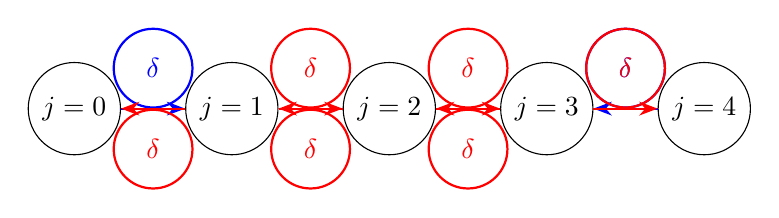
\begin{tikzpicture}[
        every node/.style={circle, draw, minimum size=1cm},
        arrow/.style={-Stealth, thick},
        delta/.style={blue, arrow},
        twodelta/.style={red, arrow}
      ]
        \node (s0) at (0,0) {$j=0$};
        \node (s1) at (2,0) {$j=1$};
        \node (s2) at (4,0) {$j=2$};
        \node (s3) at (6,0) {$j=3$};
        \node (s4) at (8,0) {$j=4$};

        % Arrows for delta (boundaries)
        \draw[delta] (s0) -- (s1) node[midway, above] {$\delta$};
        \draw[delta] (s4) -- (s3) node[midway, above] {$\delta$};

        % Arrows for 2*delta (inner strains)
        \draw[twodelta] (s1) -- (s0) node[midway, below] {$\delta$};
        \draw[twodelta] (s1) -- (s2) node[midway, above] {$\delta$};
        \draw[twodelta] (s2) -- (s1) node[midway, below] {$\delta$};
        \draw[twodelta] (s2) -- (s3) node[midway, above] {$\delta$};
        \draw[twodelta] (s3) -- (s2) node[midway, below] {$\delta$};
        \draw[twodelta] (s3) -- (s4) node[midway, above] {$\delta$};


    \end{tikzpicture}
    \caption{Biomass transfer between strains. Blue arrows (boundaries): transfer probability $\delta$. Red arrows (inner strains): $\delta$ to each neighbor, totaling $2\delta$ transfer from each inner node.}
    \label{fig:strain_transfer_example}
\end{figure}

Let $\delta = 0.2$ represent the probability that biomass shifts from one strain to a neighboring strain.

* \textbf{Strain 0 ($j=0$):}  This strain is at the boundary.  It can only lose biomass to strain 1. The fraction of biomass that remains in strain 0 is $(1 - \delta) = (1 - 0.2) = 0.8$.

* \textbf{Strain 1 ($j=1$):} This strain is in the interior. It can lose biomass to *both* strain 0 and strain 2.  It loses a fraction $\delta$ to strain 0 and a fraction $\delta$ to strain 2.  The total fraction of biomass lost by strain 1 is $2\delta = 2 \times 0.2 = 0.4$.  Therefore, the fraction of biomass that *remains* in strain 1 is $(1 - 2\delta) = (1 - 0.4) = 0.6$.

* \textbf{Strain 2 ($j=2$):}  Similar to strain 1, it loses $\delta$ to strain 1 and $\delta$ to strain 3, for a total loss of $2\delta$. The remaining fraction is $(1 - 2\delta)$.

* \textbf{Strain 4 ($j=4$):} This strain is also at a boundary. It only loses biomass to strain 3. The remaining fraction is $(1 - \delta)$.

This explains why the update equation uses $(1 - \delta)$ for the boundary strains and $(1 - 2\delta)$ for the inner strains. The $2\delta$ accounts for the biomass transferred to *both* neighboring strains.

% ... (Rest of your LaTeX document)
\subsection{Why only one delta at the ends and two deltas in the beginning? (Question and Answer)}

\textbf{Question:} Why is the biomass transfer probability $\delta$ used for the boundary strains ($j=0$ and $j=M_s$) while $2\delta$ is used for the inner strains ($j=1$ to $M_s-1$) in the update equation?  It seems like there are "more deltas in the beginning."

\textbf{Answer:} The difference between $2\delta$ inside the loop and $\delta$ at the boundaries is not about "more deltas at the beginning" but about the *number of neighbors* each strain has.

\begin{itemize}
    \item \textbf{Inner Strains ($j = 1$ to $M_s - 1$):} Each inner strain has *two* neighbors. When biomass shifts, each inner strain loses some biomass to *both* of these neighbors. If the probability of shifting to *one* neighbor is $\delta$, then the total probability of shifting biomass *away* from an inner strain is $2\delta$. That's why the update equation for inner strains uses $(1 - 2\delta)$: it represents the fraction of biomass that *remains* in the strain after transfers to *both* neighbors.

    \item \textbf{Boundary Strains ($j = 0$ and $j = M_s$):} The strains at the boundaries only have *one* neighbor. Strain $j=0$ only has a neighbor to its right (strain $j=1$), and strain $j=M_s$ only has a neighbor to its left (strain $j=M_s-1$). They can't transfer biomass "outside" the array. Therefore, they only lose biomass to *one* neighbor. The fraction of biomass lost is just $\delta$. The update equation uses $(1 - \delta)$ because only one transfer is possible.
\end{itemize}

\textbf{Analogy:} Imagine a row of people. Each person represents a strain. They're throwing balls (representing biomass) to their neighbors.

\begin{itemize}
    \item \textbf{People in the middle:} Each person in the middle throws balls to *both* the person on their left and the person on their right. They lose a total of 2 balls (if each throw has a probability of 1).
    \item \textbf{People at the ends:} The people at the ends only have *one* neighbor. They can only throw a ball to that one neighbor. They lose only 1 ball.
\end{itemize}

\textbf{In summary:} The difference between $2\delta$ inside the loop and $\delta$ at the boundaries is not about "more deltas at the beginning" but about the *number of neighbors* each strain has. Inner strains have two neighbors, so they lose biomass to both, leading to a total loss probability of $2\delta$. Boundary strains have only one neighbor, so they lose biomass to only that one neighbor, leading to a loss probability of $\delta$. This difference is essential for correctly modeling the biomass transfer at the edges of the system.
\end{document}
